\section{Introduction}
% \section{Main contributions}
% \section{Experiments}
% \section{Conclusion}

Grobid-quantities is an open-source project aiming to provide a general solution to the extraction of quantities and physical measurements from the scientific literature. 
At the time it was deployed, it represented a novel implementation based on ML, and, contrary to other works, it was not limited to specific domains or languages. 
We discuss this application as a contribution to this dissertation with particular attention to materials science, as the extraction model is implemented to support the extraction of properties from text. 

Grobid-quantities has been used in practical applications in other domains such as Earth observation data analysis~\cite{hundman2017measurement} 
Moreover, Grobid-quantities incorporates state-of-the-art machine learning (ML) techniques combined with a lexicon that is not limited to a specific subset of units~\cite{aras2014applications}.
We incorporate a normalisation process to convert measurements to the international system (SI); this step is crucial for harmonising data from various documents, even when they may use different units or formats. 
Most of the other approaches lack either the generalisation to an extensive corpus or deal mainly with specific languages. 
\cite{agatonovic2008large} addressed the identification of the numeric properties of patents using GATE (General Architecture for Text Engineering). 
\cite{am2013processing} investigated issues applied to Russian-derived languages. \cite{berrahou2013extract} described an attempt to recognise units by looking up terms from an ontology, using ML in combination with pattern matching and string metrics. 

During development, we became aware of ML-based approaches, which were limited to certain fields~\cite{dieb2015framework} or domain~\cite{kang_extracting_2013} focused on extracting measurements from experimental results in biology. 

\section{Proposed solution}
\label{sec:system}

The system accepts input in the form of text or PDF files. 
The content is extracted in a structured manner using the Grobid framework. 
Then it goes through three steps: (a) tokenisation, (b) extraction and parsing of measurements, and (c) normalisation of quantities.

\subsection{Data model}
\label{subsec:data-model}

The data model (Figure \ref{fig:data-model-schema-2}) was based on the concept of \textit{Measurement}, which links an object or a substance with one or more \textit{quantities}. 
We defined four \textit{Measurements} types: (a) atomic, in case of a single measurement (e.g., 10 grams). (b) interval (\textit{from 3 to 5 km}) and (c) range ($100 \pm 4$ mm) for continuous values, and (d) a list of discrete values. A \textit{Quantity} links the quantitative value and the unit. 

\label{subsub:data-model}
\begin{figure}[htbp]
  \centering
  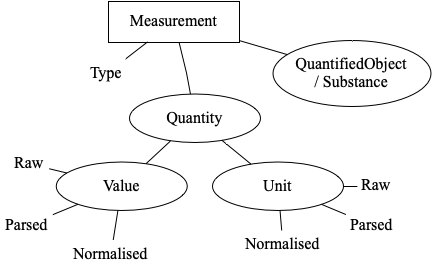
\includegraphics[width=0.8\linewidth]{figures/quantities/schema-2.png}
  \caption{Schema of the data model, from the data parsing and normalisation point of view.}
  \label{fig:data-model-schema-2}
\end{figure}

Since data extracted from PDF documents unavoidably present irregular tokens from incorrect UTF-8 encoding or missing fonts, we designed this model to allow partial results. 
The \textit{Value} and \textit{Unit} entities allow three different representations (Figure \ref{fig:data-model-schema-2}): \textit{Raw} as appear in input, \textit{Parsed} unifies the value into the numerical expression, and the unit with its properties (system, type). Finally, \textit{Normalised} contains the transformed unit and values to the SI system. \textit{Value} object supports four types of representations: numeric (2, 1000), alphabetic (two, thousand), scientific notation ($3\cdot10\textsuperscript{5}$), and time, which is also an expression of measurement. Units objects are organised following the SI, which allows representing units as products of simpler compounds (e.g. m/s to $m \cdot s\textsuperscript{-1}$) further decomposed as triples (prefix, base and power).

\subsection{Tokenisation}
This process splits the input data into tokens. Grobid-quantities uses a two-phase tokenisation: (1) first it splits by punctuation marks, then (2) each resulting token is re-tokenised to separate adjacent digits and alphanumeric characters. Given the example \texttt{25m\^{}2}, first returns a list \texttt{[25m, \^{}, 2]} and then recursively divides \texttt{25m} as \texttt{[25, m]}  resulting in \texttt{[25, m, \^{}, 2]}.

\subsection{Extraction}
% Quantity model 
The tokens are passed through three ML models, in cascade: first the \textit{Quantities} parser determines the appropriate unit and value tags. The results are further processed by the respective \textit{Units} and \textit{Values} parsers as illustrated in Figure \ref{fig:schema-cascade}.  

\begin{figure}[htbp]
  \centering
  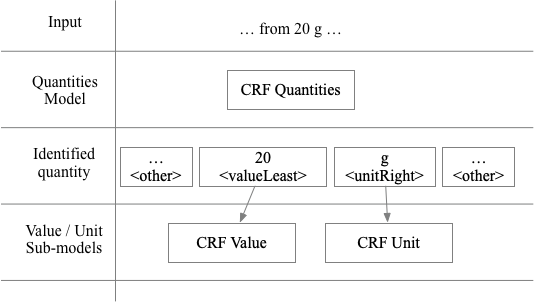
\includegraphics[width=\linewidth]{figures/quantities/schema-cascade}
  \caption{The cascade approach of the applied parsers. The Quantities parser recognises value and units which are passed, respectively, to Values and Units parsers for further extraction.}
  \label{fig:schema-cascade}
\end{figure}

Table \ref{tab:quantities-model-labels} describes the labels predicted by \textit{Quantities} parser. Note that to reconstruct complex structured objects from the flat sequence generated by the engine, additional labels are necessary (such as \texttt{<unitLeft>}, \texttt{<unitRight>}, for units).

\begin{table}[htbp]
\centering
  \caption{Labels description for the Quantities parser. In bold are highlighted the value referred by the label.}
  \label{tab:quantities-model-labels}
  \begin{tabular}{lll}
    \toprule
    Label & Description & Example\\
    \midrule
    \texttt{<valueAtomic>} & value of an atomic quantity & \textbf{2} m \\
    \texttt{<valueLeast>} & least value in an interval & from \textbf{2} m \\
    \texttt{<valueMost>} & max value in an interval & up to \textbf{7} m \\
    \texttt{<valueBase>} & base value in a range & $\textbf{20}\pm7$ m \\
    \texttt{<valueRange>} & range value in a range & $20 \pm \textbf{7}$ m \\
    \texttt{<valueList>} & list of quantities & \textbf{2}, \textbf{3} and \textbf{10} m \\
    \texttt{<unitLeft>} & left-attached unit & \textbf{pH} 2 \\
    \texttt{<unitRight>} & right-attached unit & 2 \textbf{m} \\
    \texttt{<other>} & everything else & - \\
  \bottomrule
\end{tabular}
\end{table}

% Gazetteers
Previous work presented extensive use of databases or ontologies. In our solution, we used a similar approach. We created a list of units (in English, French, and German) with their characteristics: system (SI base, SI derived, imperial, etc.) and type (volume, length, etc.) and their representations: notations (m\textsuperscript{3}, \texttt{m\^{}3}), lemmas (cubic meter, cubic metre) and inflexions (cubic meters, cubic metres). We made this list available through the \textit{Unit Lexicon}, which offers unit lookups by properties (such as notation, lemma, and inflexion). A second gazetteer was created to allow the transformation of alphabetic values into numeric ones (for example, 21 to 21).

Features in the \textit{Quantities} model are generated from preceding and following tokens, presence of capital, digits. Orthogonal features are obtained through the \textit{Unit Lexicon}, like a \textit{Boolean} indicating whether a token is a known unit or not. Typographical information (such as format, fonts, subscript and superscript) are ignored. 

% Unit model 
The \textit{Units} parser works at character level and uses the \textit{Unit Lexicon} to highlight known units or prefixes. The input tokens are parsed and transformed into a product of triples (prefix, base, power) as shown in Table \ref{tab:units-model-labels}. For example, \texttt{ Kg / mm\textsuperscript{2}}, corresponds to \texttt{$Kg\cdot mm\textsuperscript{-2}$} and becomes \texttt{[(K, g, 1), (m, m, -2)]} as a product of triples. We define "simple units" all the units that can be decomposed in a single triplet, and complex unit when they are decomposed in multiple triplets. 

\begin{table}[htbp]
\centering
  \caption{Labels description for the Units parser. In bold are highlighted specific examples. }
  \label{tab:units-model-labels}
  \begin{tabular}{lll}
    \toprule
    Label & Description & Example\\
    \midrule
    \texttt{<prefix>} & prefix of the unit  & \textbf{k}m\textsuperscript{2} \\
    \texttt{<base>} & unit base & k\textbf{m}\textsuperscript{2}\\
    \texttt{<pow>} & unit power & km\textsuperscript{\textbf{2}}\\
    \texttt{<other>} & everything else & - \\
  \bottomrule
\end{tabular}
\end{table}

We then use the structured triples to fetch the corresponding information (system, type) from the \textit{Unit Lexicon} and attach them to the resulting object. 
This implementation processes the unit characters in right-to-left order. 
%Priority modifiers, such as parenthesis, are ignored because more complex to manage and not frequent. 
Priority modifiers, such as parentheses, are ignored. They are generally not frequent in unit expressions and require a more complex logic.

In parallel, the \textit{Values} parser unifies the format of the identified values into numerical formats. It supports four types: numeric, alphabetic, scientific notation, and time expression (see Table \ref{tab:values-model-labels}). Different techniques are applied for each type: alphabetic expressions are looked up in the word-to-number gazetteer, and scientific notation is parsed and calculated mathematically. Time expressions are further segmented using the Grobid built-in "Date" model.

\begin{table}[htbp]
\centering
  \caption{Labels description for the Values parser. In bold are highlighted specific examples.}
  \label{tab:values-model-labels}
  \begin{tabular}{lll}
    \toprule
    Label & Description & Example\\
    \midrule
    \texttt{<number>} & numeric value / coefficient & $\textbf{2.5}\cdot10\textsuperscript{\textbf{5}}$ \\
    \texttt{<alpha>} & alphabetic value & \textbf{twenty} \\
    \texttt{<time>} & time expression  & in \textbf{1970-01-02}\\
    \texttt{<base>} & base in scientific notation & $2.5\cdot\textbf{10}\textsuperscript{5}$\\
    \texttt{<pow>} & exponent in scientific notation & $2.5\cdot10\textsuperscript{\textbf{5}}$ \\
    \texttt{<other>} & everything else & - \\
  \bottomrule
\end{tabular}
\end{table}

\subsection{Normalisation}

The measurements extracted are transformed to the base SI unit (grams to kg, Celsius to Kelvin, etc.). We used an external Java library called Units of Measurement~\cite{units_of_measurement}, which provides a set of standard interfaces and implementations to safely handle units and quantities. Manipulation of measurements with transformations often leads to common errors due to wrong rounding and approximations. 

\section{Evaluation and results}
\label{sec:results}

We trained and evaluated our system's models using a dataset based on 32 scientific publications (English, Open Access (OA)) and three patents (with translation in English, French, and German) randomly selected from different domains such as medicine, robotics, astronomy, and physiology. 
Training data was generated automatically and then corrected and cross-checked by three annotators. The dataset was then divided into two parts for training (26 documents) and evaluation (9 documents).
We use the holdout dataset partition to evaluate each model and produce precision, recall, and f1 scores, as summarised in Tables~\ref{tab:evaluation-quantities-holdout},~\ref{tab:evaluation-units-holdout}, and~\ref{tab:evaluation-values-holdout}. 
As presented in Chapter~\ref{cha:extraction-experimental-data}, we report the results of four architectures: CRF, RNN (with and without layout features), and transformers, fine-tuning a pre-trained SciBERT~\cite{Beltagy2019SciBERT}. 

\begin{table}[htbp]
    \centering\small
    \caption{Evaluation scores (\%) of the Quantities ML model with holdout set. Support (Supp) indicates the number of labels in the training data. Values in bold indicate the highest score. P: precision, R: recall. Results for deep learning results are average over five independent runs of training and evaluation. }

    \scalebox{0.6}{
    \begin{tabular}{l ccc ccc ccc ccc r}
        \toprule
        \textbf{Label}         & \multicolumn{3}{c}{\textbf{CRF}} & \multicolumn{3}{c}{\textbf{BidLSTM\_CRF}} & \multicolumn{3}{c}{\makecell{\textbf{BidLSTM\_CRF}                                                                                                                                                 \\\textbf{\_FEATURES}}} &  \multicolumn{3}{c}{\textbf{SciBERT}} & \textbf{Supp}  \\
        \cmidrule(lr){2-4}\cmidrule(lr){5-7}\cmidrule(lr){8-10}\cmidrule(lr){11-13}\cmidrule(lr){14-14}
                               & \textbf{P}                       & \textbf{R}                                & \textbf{F1}                                        & \textbf{P} & \textbf{R} & \textbf{F1}    & \textbf{P}     & \textbf{R} & \textbf{F1}    & \textbf{P} & \textbf{R}     & \textbf{F1}    &      \\
        \midrule
        \texttt{<unitLeft>} & 88.74 & 83.19 & 85.87 & 88.56 & 92.07 & 90.28 & 88.91 & \textbf{92.20} & 90.53 & \textbf{93.99} & 90.30 & \textbf{92.11} & 464 \\
        \texttt{<unitRight>} & \textbf{30.77} & 30.77 & 30.77 & 24.75 & \textbf{30.77} & 27.42 & 21.73 & 30.77 & 25.41 & 21.84 & \textbf{36.92} & \textbf{27.44} & 13 \\
        \texttt{<valueAtomic>} & 76.29 & 78.66 & 77.46 & 78.14 & 86.06 & 81.90 & 78.21 & 86.20 & 82.01 & \textbf{84.50} & \textbf{88.19} & \textbf{86.31} & 581\\
        \texttt{<valueBase>} & 84.62 & 62.86 & 72.13 & 83.51 & 94.86 & 88.61 & 83.36 & \textbf{97.14} & 89.72 & \textbf{100.00} & 90.86 & \textbf{95.20} & 35 \\
        \texttt{<valueLeast>} & 77.68 & 69.05 & 73.11 & \textbf{82.14} & 60.63 & 69.67 & 80.73 & 60.63 & 69.12 & 81.09 & \textbf{71.59} & \textbf{76.04} & 126 \\
        \texttt{<valueList>} & 45.45 & 18.87 & 26.67 & 62.15 & 10.19 & 17.34 & \textbf{73.33} & 8.68 & 15.33 & 64.12 & \textbf{43.78} & \textbf{51.64} & 53\\
        \texttt{<valueMost>} & 71.62 & 54.64 & 61.99 & 77.64 & 68.25 & 72.61 & 77.25 & \textbf{70.31} & 73.58 & \textbf{81.52} & 67.42 & \textbf{73.71} & 97\\
        \texttt{<valueRange>} & \textbf{100.00} & 97.14 & 98.55 & 96.72 & \textbf{100.00} & \textbf{98.32} & 94.05 & 98.86 & 96.38 & 99.39 & 91.43 & 95.24 & 35\\
        \midrule
        \textbf{All (micro avg.)} & 80.08 & 75 & 77.45 & 81.81 & 81.73 & 81.76 & 81.76 & 81.94 & 81.85 & \textbf{86.24} & \textbf{83.96} & \textbf{85.08} & \\
        \bottomrule
    \end{tabular}
    }
    
    \label{tab:evaluation-quantities-holdout}
\end{table}


% Scores + discussion Quantities CRF model 
The best results of the Quantities ML models were achieved by the SciBERT model, for which we recorded an F1 micro-average of 85.14\% with precision and recall of 86.24\% and 83.96\%, respectively. SciBERT outperforms the CRF model by 8\% F1-score.  
With RNN, we confirmed the same observation reported in Chapter~\ref{cha:extraction-experimental-data}, that layout orthogonal features are not used, or their use does not "help" the model to better generalise. 
In general, SciBERT performs better than any other model in most labels, only recognising \texttt{<valueRange>} result in a a better F1-score by the CRF model. 
The support information also suggest that \texttt{<list>} and \texttt{<unitRight>} require more training examples.

% Scores + discussion Unit CRF model 
Unit expressions are generally short (1-3 characters) and with lower variability, which means that each label tends to be more duplicates than in the training datasets of other models. 
For example, the expressions 1\% and 2\% have two different values (1, 2) and the same unit (\%), which would appear twice. 
For this reason, we evaluated the unit ML model with a separate dataset of 2000 annotated units~\cite{foppiano2019leveraging} that were initially automatically extracted from 3490 articles in the Journal of Applied Physics~\cite{suzuki2018constructing}.
After annotating each unit following the schema discussed in Table~\ref{tab:units-model-labels}, the resulting corpus contains approximately 700 simple and 1300 complex units. 
As illustrated in Table~\ref{tab:evaluation-units-holdout}) the overall scores for the Units ML model are lower, because the evaluation corpus is larger than the training corpus and contains a substantial percentage of complex units, while in the training dataset the complex units are less frequent.  
Interestingly, Table~\ref{tab:evaluation-units-holdout} shows that the orthogonal features become relevant and the best scores are obtained by the RNN with features BidLSTM\_CRF\_FEATURES and the CRF. 

\begin{table}[htbp]
    \centering\small
    \caption{Evaluation scores (\%) of the Units ML model with holdout set. Support (Supp) indicates the number of labels in the training data. Values in bold indicate the highest score. P: precision, R: recall.}

    \scalebox{0.6}{
    \begin{tabular}{l ccc | ccc | ccc | ccc r}
        \toprule
        \textbf{Label}         & \multicolumn{3}{c}{\textbf{CRF}} & \multicolumn{3}{c}{\textbf{BidLSTM\_CRF}} & \multicolumn{3}{c}{\makecell{\textbf{BidLSTM\_CRF}                                                                                                                                                 \\\textbf{\_FEATURES}}} &  \multicolumn{3}{c}{\textbf{SciBERT}} & \textbf{Supp}  \\
        \cmidrule(lr){2-4}\cmidrule(lr){5-7}\cmidrule(lr){8-10}\cmidrule(lr){11-13}\cmidrule(lr){14-14}
                               & \textbf{P}                       & \textbf{R}                                & \textbf{F1}                                        & \textbf{P} & \textbf{R} & \textbf{F1}    & \textbf{P}     & \textbf{R} & \textbf{F1}    & \textbf{P} & \textbf{R}     & \textbf{F1}    &      \\
        \midrule
        \texttt{<base>} & \textbf{80.57} & \textbf{82.34} & \textbf{81.45} & 56.01 & 50.34 & 53.02 & 59.98 & 56.33 & 58.09 & 61.41 & 57.08 & 59.16 & 3228\\
        \texttt{<pow>} & 72.65 & \textbf{74.45} & 73.54 & 93.70 & 62.38 & 74.88 & \textbf{93.71} & 68.40 & \textbf{78.94} & 91.24 & 64.60 & 75.60 & 1773 \\
       \texttt{<prefix>} & 93.8 & 84.69 & \textbf{89.02} & 80.31 & 85.25 & 82.54 & 83.21 & 83.58 & 83.35 & 82.10 & 85.30 & 83.62 & 1287\\
        \midrule
        \textbf{All (micro avg)} & \textbf{80.73} & 80.6 & 80.66 & 70.19 & 60.88 & 65.20 & 73.03 & \textbf{65.31} & \textbf{68.94} & 73.02 & 64.97 & 68.76 & \\
        \bottomrule
    \end{tabular}
    }
    
    \label{tab:evaluation-units-holdout}
\end{table}


% Scores + discussion Values CRF model 
The Value ML model scores are shown in Table~\ref{tab:evaluation-values-holdout}, and show that SciBERT outperforms the other architectures in almost all labels. SciBERT obtains an F1 score of 99.23\%, with 99.13\% and 99.33\% in precision and recall, respectively.
We noticed that both \textit{<base>}, \textit{<pow>} and \textit{<time>} have lower f1-score. While \textit{<base>} and \textit{<pow>} require more training data, \textit{<time>} expressions may overlap with \textit{<number>} suggesting more contextual information should be introduced. 

\begin{table}[htbp]
    \centering\small
    \caption{Evaluation scores (\%) of the Values ML model with holdout set. Support (Supp) indicates the number of labels in the training data. Values in bold indicate the highest score. P: precision, R: recall.}

    \scalebox{0.6}{
    \begin{tabular}{l ccc | ccc | ccc | ccc | r}
        \toprule
        \textbf{Label}         & \multicolumn{3}{c}{\textbf{CRF}} & \multicolumn{3}{c}{\textbf{BidLSTM\_CRF}} & \multicolumn{3}{c}{\makecell{\textbf{BidLSTM\_CRF}                                                                                                                                                 \\\textbf{\_FEATURES}}} &  \multicolumn{3}{c}{\textbf{SciBERT}} & \textbf{Supp}  \\
        \cmidrule(lr){2-4}\cmidrule(lr){5-7}\cmidrule(lr){8-10}\cmidrule(lr){11-13}\cmidrule(lr){14-14}
                               & \textbf{P}                       & \textbf{R}                                & \textbf{F1}                                        & \textbf{P} & \textbf{R} & \textbf{F1}    & \textbf{P}     & \textbf{R} & \textbf{F1}    & \textbf{P} & \textbf{R}     & \textbf{F1}    &      \\
        \midrule
        \texttt{<alpha>} & 98.06 & 96.03 & 92.02 & 97.67 & \textbf{99.53} & 98.58 & 97.82 & \textbf{99.53} & 98.66 & \textbf{98.59} & \textbf{99.53} & \textbf{99.05}  & 126 \\
        \texttt{<base>} & \textbf{99.91} & 92.31 & \textbf{96.00} & 96.92 & 92.31 & 94.52 & 96.92 & 93.85 & 95.32 & 90.40 & \textbf{98.46} & 92.88  &13 \\
        \texttt{<number>} & 97.50 & \textbf{99.88} & 98.36 & 99.24 & 99.34 & 99.29 & 99.21 & 99.38 & 99.30 & 99.48 & 99.31 & \textbf{99.40}  & 811 \\
        \texttt{<pow>} & \textbf{100.00} & \textbf{100.00} & \textbf{100.00} & 92.92 & 92.31 & 92.47 & 90.28 & 93.85 & 91.90 & \textbf{100.00} & \textbf{100.00} & \textbf{100.00}  & 13 \\
        \midrule
        \textbf{All (micro avg)} & 95.79 & 99.27 & 97.50 & 98.90 & 99.17 & 99.03 & 98.86 & 99.25 & 99.05 & \textbf{99.13} & \textbf{99.33} & \textbf{99.23} & \\
        \bottomrule
    \end{tabular}
    }
    
    \label{tab:evaluation-values-holdout}
\end{table}


% \clearpage
% \begin{sidewaystable}[htbp]
%   \centering\small
%   \caption{}
%   \scalebox{0.6}{
%       \begin{tabular}{lccccccccccccc}
%         \toprule
%         Label & \textbf{Scibert} & \textbf{MatBERT} & \textbf{MatsciBERT} & \textbf{batteryonlyBERT} & \textbf{batterysciBERT} & \textbf{batteryBERT} & \textbf{BERT} & \textbf{\makecell{BioLinkBERT\\(base)}} & \textbf{MaterialsBERT} & \textbf{\makecell{BiomedNLP-\\PubMedBERT}} & \textbf{cs\_roberta\_base} & \textbf{\makecell{biomed\_roberta\\(base)}} & \textbf{ChemBERT} \\
%         \midrule
%         \texttt{<unitLeft>} & 92.11 & 92.27 & 91.80 & 92.50 & 91.34 & 91.60 & 90.19 & 91.55 & 90.23 & 91.33 & 89.32 & 90.85 & 88.80 \\
%         \texttt{unitRight} & 27.44 & 28.43 & 28.84 & 33.33 & 25.61 & 32.59 & 32.07 & 24.42 & 32.23 & 25.12 & 27.60 & 30.87 & 39.78\\
%         \texttt{valueAtomic} & 86.31 & 85.37 & 83.44 & 85.34 & 85.10 & 83.92 & 79.33 & 85.02 & 84.24 & 86.53 & 82.90 & 83.52 & 79.48\\
%         \texttt{valueBase} & 95.20 & 93.63 & 91.75 & 92.18 & 93.25 & 94.33 & 89.04 & 95.24 & 88.68 & 95.24 & 93.54 & 92.85 & 84.53\\
%         \texttt{valueLeast} & 76.04 & 74.83 & 74.99 & 76.78 & 75.69 & 74.87 & 73.12 & 78.66 & 75.44 & 77.01 & 79.88 & 82.32 & 68.92\\
%         \texttt{valueList} & 51.64 & 60.41 & 50.07 & 56.65 & 50.90 & 59.79 & 41.21 & 52.48 & 48.25 & 55.22 & 55.21 & 52.95 & 39.55\\
%         \texttt{valueMost} & 73.71 & 72.40 & 70.45 & 71.88 & 74.37 & 71.29 & 59.84 & 74.54 & 69.69 & 75.17 & 71.77 & 76.00 & 62.15\\
%         \texttt{valueRange} & 95.52 & 95.52 & 94.96 & 95.52 & 95.52 & 95.52 & 93.66 & 95.52 & 95.24 & 95.52 & 95.52 & 94.97 & 81.93\\
%         \midrule
%         \textbf{All (micro avg.)} & 85.08 & 84.82 & 83.23 & 84.87 & 84.26 & 83.92 & 79.72 & 84.39 & 83.00 & 85.12 & 82.88 & 84.05 & 78.82\\
%         \bottomrule
%       \end{tabular}
%     }
% \end{sidewaystable}
% \clearpage

\section{Conclusions}

In this contribution, we highlight our Parser for measurements and physical quantities. Although our dissertation discusses a novel application to materials science, we present a tool that is not limited to just that. 
This contribution is partially reused for our materials science project; however, its application is extensively applied in biology~\cite{hundman2017measurement}
and other disciplines. 

This contribution was published in the paper "Automatic identification and normalisation of physical quantities from scientific literature"~\cite{foppiano2019quantities}.